

%\newcommand*{\ACM}{}%

\ifdefined\ACM

%\documentclass[sigplan,screen]{acmart}
\documentclass[manuscript,screen,review]{acmart}

\else
\documentclass{article}
\usepackage[utf8]{inputenc}
\usepackage[a4paper, total={6in, 9in}]{geometry}
\usepackage{braket}
\usepackage{xcolor}
\usepackage{amsmath}
\usepackage{amsfonts}
\usepackage{amsthm}
\usepackage{amssymb}
%\usepackage[ocgcolorlinks]{hyperref}
\usepackage{hyperref}
%\usepackage{hyperref,xcolor}
%\usepackage[ocgcolorlinks]{ocgx2}
\usepackage{cleveref}
\usepackage{graphicx}
\usepackage{svg}
\usepackage{float}
\usepackage{tikz}
\usetikzlibrary{patterns, shapes.arrows}
\usepackage{adjustbox}
%\usepackage{tikz-network}
\usepackage{tkz-graph}
\usepackage{tkz-berge}
\usepackage[linesnumbered]{algorithm2e}
\usepackage{multicol}
\usepackage[backend=biber,style=alphabetic,sorting=ynt]{biblatex}
%\usepackage{xcolor}
%\usepackage{tkz-berge}
%\usepackage{tkz-graph}
\usepackage{pgfplots}
\usepackage{sagetex}
\usepackage{setspace}
\usepackage{etoc}
%\usepackage{wrapfig}
\usepackage{pgfgantt}
\DeclareUnicodeCharacter{2212}{−}
\usepgfplotslibrary{groupplots,dateplot}
\pgfplotsset{compat=newest}

\newtheorem{theorem}{Theorem}
\newtheorem{definition}{Definition}
\newtheorem{example}{Example}
\newtheorem{claim}{Claim}
\newtheorem{fact}{Fact}
\newtheorem{remark}{Remark}
\newtheorem*{theorem*}{Theorem}
\newtheorem{lemma}{Lemma}
\crefname{lemma}{Lemma}{Lemmas}
\hypersetup{colorlinks=true}
% , allcolors=blue,allbordercolors=blue,pdfborderstyle={0 0 1}}
%\hypersetup{pdfborder={2 2 2}}
% pdfpagemode=FullScreen,
% backref 

\newtheorem{problem}{Problem}
\crefname{problem}{Problem}{Problems}

\DeclareMathOperator{\Ima}{Im}


\addbibresource{sample.bib} %Import the bibliography file

\fi
\begin{document}

\newcommand{\commentt}[1]{\textcolor{blue}{ \textbf{[COMMENT]} #1}}
\newcommand{\ctt}[1]{\commentt{#1}}
\newcommand{\prb}[1]{ \mathbf{Pr} \left[ {#1} \right]}
\newcommand{\onotation}[1]{\(\mathcal{O} \left( {#1}  \right) \)}
\newcommand{\ona}[1]{\onotation{#1}}
%\newcommand{\PSI}{{\ket{\psi}}}
%\newcommand{\LESn}{\ket{\psi_n}}
%\newcommand{\LESa}{\ket{\phi_n}}
%\newcommand{\LESs}{\frac{1}{\sqrt{n}}\sum_{i}{\ket{\left(0^{i}10^{n-i}\right)^{n}}}}
%\newcommand{\Hn}{\mathcal{H}_{n}}
%\newcommand{\Ep}{\frac{1}{\sqrt{2^n}}\sum^{2^n}_{x}{ \ket{xx}}}
%\newcommand{\HON}{\ket{\psi_{\text{honest}}}}
%\newcommand{\Lemma}{\paragraph{Lemma.}}
\newcommand{\Cpa}{[n, \rho n, \delta n]}
%\setlength{\columnsep}{0.6cm}
\newcommand{\Jvv}{ \bar{J_{v}} } 
\newcommand{\Cvv}{ \tilde{C_{v}} } 

\newcommand{\Gz}{ G_{z}^{\delta} } 
\newcommand{ \Tann } {  \mathcal{T}\left( G, C_0 \right) }


\title{Removing The $w$-Robustness Assumptions.} 
\author{David Ponarovsky}

\ifdefined\ACM
\affiliation{%
  \institution{The Th{\o}rv{\"a}ld Group}
  \streetaddress{1 Th{\o}rv{\"a}ld Circle}
  \city{Hekla}
  \country{Iceland}}
\email{larst@affiliation.org}
\else
\maketitle
\fi

\abstract{We propose an alternative simple construction of good LTC codes. In contrast to previews, constructions made by \cite{Dinur}, \cite{leverrier2022quantum} and \cite{Pavel}, our construction doesn't require spicel properties of the small codes, such as $w$-robustness and $p$-resistance for puncturing.  
} 


\ifdefined\ACM
\maketitle
\fi
%\begin{multicols*}{2}
\section{Preambles}

Localy Testable Codes, or LTC, are error correction codes such that verfining a uinformly random cchoosen check, would be enough to detect any error with probability proportional to it's size. Bisdes the clear computional adventage they offer, they took roles at the eriler PCP proofs.  
  In this work, we propose a new construction for good LTC codes, which also have a good testability parameter. In the sense   Our proof also indirectly answers the following question. Why most of the good LDPC codes are known to be bad in terms of detecting errors? In other words, It seems that for most of them, there exist strings that are very far from being in the code and, meanwhile, fail to satisfy only a small number of restrictions.
  While the previous LDPC constructions focused on ensuring that the yielded code would have a good rate and distance parameters, our construction enforces the restrictions collection to have a nontrivial fraction of degeneration. That is, removing a single restriction will not change the code, as any restriction is linearly dependent on the others.



      \section{Introduction}
  \section{Introduction.}
.. bla bla bla.. bla bla ..     
\definition[General Entanglement State]{ We say that $\PSI$ is general entanglement \label{def:gEnt} if .. }

\definition[Local-Measure-Circuit] { We say that a quantum circuit $C$ is a local measure circuit \label{def:lmc} if it's can be described as a decomposition of poly classical circuit and a constant depth quantum circuit which contains only 1-qubit gates and measurements. 

We would think about local measure circuits as chip circuits. }

\definition[$p_{0}-\Delta$ Fault Tolerance Circuit]{ We say that $\mathcal{C}$ is $p_{0}-\Delta$ fault tolerance \label{def:gft} presentation of abstract circuit $C$ if there exists a local measure circuit $C_{0}$ \ref{lmc} such it's grunted that for noise $p < p_{0}$ $\mathcal{C}$ compute $C$ w.h.p,
And in addition, if $p \in \left( p_{0}, p_{0} + \varepsilon \right)$ then by applying a $C_{0}$ on $\mathcal{C}$ output yields a general entanglement state \label{def:gEnt}}       

\ctt{We would like to add a complexity parameter for the above definition, for example, ``a general entanglement state over more than $\frac{1}{5}$ of the qubits.}  

  %Linear Error Correction Codes, 
  \subsection{Notations, Definitions, And Our Contribution}
  Here we focus only on linear binary codes, which one could think about as linear subspaces of $\mathbb{F}_{2}^{n}$. A common way to measure resilience is to ask how many bits an evil entity needs to flip such that the corrupted vector will be closer to another vector in that space than the original one. Those ideas were formulated by Hamming \cite{Hamming}, who presented the following definitions. 
  \begin{definition} \label{bi-code} Let $n \in \mathbb{N}$ and $\rho, \delta\in \left( 0,1 \right)$. We say that $C$ is a \textbf{binary linear code} with parameters $[n, \rho n, \delta n]$. If $C$ is a subspace of $\mathbb{F}_{2}^{n}$, and the dimension of $C$ is at least $\rho n$. In addition, we call the vectors belong to $C$ \textit{codewords} and define the distance of $C$ to be the minimal number of different bits between any codewords pair of $C$.   
  \end{definition}
  From now on, we will use the term code to refer to linear binary codes, as we don't deal with any other types of codes. Also, even though it is customary to use the above parameters to analyze codes, we will use their percent forms called the relative distance and the rate of code, matching $\delta$ and $\rho$ correspondingly.     
  \begin{definition} \label{family} A \textbf{family of codes} is an infinite series of codes. Additionally, suppose the rates and relative distances converge into constant values $\rho,\delta$. In that case, we abuse the notation and call that family of codes a code with $[n, \rho n, \delta n]$ for fixed $\rho, \delta\in [ 0,1 )$, and infinite integers $n \in \mathbb{N}$.     
  \end{definition}
  Notice that the above definition contains codes with parameters attending to zero. From a practical view, it means that either we send too many bits, more than a constant amount, on each bit in the original message. Or that for big enough $n$, adversarial, limited to changing only a constant fraction of the bits, could disrupt the transmission. That distinction raises the definition of good codes.

  \begin{definition} \label{good-code} We will say that a family of codes is a \textbf{good code} if its parameters converge into positive values. 
  \end{definition}

  \ifdefined\LDPCLTC
    Apart from distance and rate here, we interest also that the checking process will be robust. In particular,  we wish that against significant errors, forgetting to perform a single check will sabotage the entire computation only with a tiny probability.  
  \begin{definition} \label{LTC} Consider a code $C$  a string $x$, and denote by $\xi\left( x \right)$ the fraction of the checks in which $x$ fails. $C$ will be called a \textbf{local-testability $f\left( n \right)$} If there exists $\kappa > 0$ such that 
  \begin{equation*}
    \begin{split}
      \frac{d\left( x, C \right)}{n} \le \kappa \cdot  \xi\left( x \right) f\left( n \right)
    \end{split}
  \end{equation*}
\end{definition}
 
 %
\fi

  
\ifdefined\LDPCLTC
  Now, we are ready to formulate our contribution. 

  Nowadays, we are aware of a wide range of constructions yield good codes, including the expander codes of Sipser and Spilman \cite{ExpanderCodes} and the LTC codes of Dinur \cite{Dinur}, \cite{Pavel}, \cite{leverrier2022quantum}. Thus if a decade ago, the main question was the existence of a good code and its construction, now, and particularly in this work, we concentrate on getting a deep understanding of what makes those constructions work. By utilizing those insights, we succussed in achieving significantly simpler construction. Our results: 

 \begin{theorem*}[Theorem 1] There exist a constant $\alpha > 0$ and an infinte family of Tanner Codes $C = \Tann$ such that any ireducable codeword $x$ of a coresponding disagreement code $x \in C_{\oplus}$ at length $n$, weight at least $\alpha n$. \end{theorem*}

\begin{theorem*}[Theorem 1+] There exist a constant $\alpha > 0 $ and infinite familiy of codes which satesfies Theroem 1 and also good.
  \end{theorem*}



\fi

  \subsection{Singleton Bound}  
  To get a feeling of the behavior of the distance-rate trade-of, Let us consider the following two codes; each demonstrates a different extreme case. First, define the repetition code $C_{r} \subset \mathbb{F}_{2}^{n \cdot r}$, In which, for a fixed integer $r$, any bit of the original string is duplicated $r$ times. Second, consider the parity check code $C_{p} \subset \mathbb{F}_{2}^{n+1}$, in which its codewords are only the vectors with even parity. Let us analyze the repetition code. Clearly, any two $n$-bits different messages must have at least a single different bit. Therefore their corresponding encoded codewords have to differ in at least $r$ bits. Hence, by scaling $r$, one could achieve a higher distance as he wishes. Sadly the rate of the code decays as $n/nr = 1/r$. In contrast, the parity check code adds only a single extra bit for the original message. Therefore scaling $n$ gives a family which has a rate attends to $\rho \rightarrow 1$. However, flipping any two different bits of a valid codeword is conversing the parity and, as a result, leads to another valid codeword.

  To summarize the above, we have that, using a simple construction, one could construct the codes $[r, 1, r]$, $[r, r-1, 2]$. Each has a single perfect parameter, while the other decays to the worst.\ifdefined\LDPCLTC In the next section, we will review the Singleton bound, which states that for any code (not necessarily good), there must be a zero-sum game between the relative distance and the rate.
\fi % 

  Besides being the first bound, Singleton bound demonstrates how one could get results by using relatively simple elementary arguments. It is also engaging to ask why the proof yields a bound that, empirically, seems far from being tight.
  \begin{theorem*}[Singleton Bound.]\label{theorem*:Sing}  For any linear code with parameter $[n,k,d]$, the following inequality holds:
  \begin{equation*}
    k+ d \le n + 1
  \end{equation*} 
  \end{theorem*}

\begin{proof} Since any two codewords of $C$ differ by at least $d$ coordinates, we know that by ignoring the first $d-1$ coordinate of any vector, we obtain a new code with one-to-one corresponding to the original code. In other words, we have found a new code with the same dimension embedded in $\mathbb{F}_{2}^{n-d+1}$. Combine the fact that dimension is, at most, the dimension of the container space, we get that:  
  \begin{equation*}
    \begin{split}
      \dim C &= 2^{k} \le 2^{n-d+1} \Rightarrow k+d \le n + 1
    \end{split}
  \end{equation*}
\end{proof}

It is also well known that the only binary codes that reach the bound are: $[n,1,n]$, $[n,n-1,2]$,$[n,n,1]$ \cite{eczoo_mds}. In particular, there are no good binary codes that obtain equality(And no binary code which get close to the equality exits). Let's review the polynomial code family \cite{Reed1960PolynomialCO}, which is a code over none binary field that achieve the Singleton Bound. 

\ifdefined\LDPCLTC
\subsection{Polynomial Code.} Consider the field $\mathbb{F}_{m}$ for an arbitrary prime power $m=q^{l}$ greater than $n$. The polynomial codes relay on the fact that any two different polynomials in the ring $\mathbb{F}_{m}\left[ x \right]$ at degree at most $d$ different by at least $m - d + 1$ points. For example consider a polynomials pair at degree 1, namely two linear straight lines. If they are not identical than they have at most single intersection point, and the disagree on each of the $n-1$ remaining points.  

So by define the code to be the subspace contains all the polynomials at degree at most $d$, in such way that any codeword is an image of such polynomail encoded by $n$ numbers, one can garntee a lower bound on the code's distance. Formally we define:     
\begin{definition}[Polynomial Code. \cite{Reed1960PolynomialCO}]
  Fix $m > n $ to be a prime power and let $a_{0},a_{1},a_{2},\ldots a_{n}$ distinct points of the field $\mathbb{F}_{m} = R$  and define the code $C \subset R $ as follows:  
  \begin{equation*}
    \begin{split}
      C = \left\{p\left(a_{0}\right),p\left(a_{1}\right),p\left(a_{2}\right),\cdots p\left(a_{n}\right) : p \text{ is polynomial at degree at most } d \right\}
    \end{split}
  \end{equation*}
\end{definition}
Observe that $C$ is a linear code at length $n$ over the aleph-bet $\mathbb{F}_{m}$. The following Lemma states the realtion between the maximal degree of the polynomials and the properites of the code.   
\begin{lemma}
  Fix the degree of the polynomial code to be at most $d$. Then the parameters of the code are $[n,d + 1, n - d]$.  
  \label{polycode}
\end{lemma}
\begin{proof}
  The dimension of the code equals to the dimension of the polynomials space at degree at most $d$ which is spanned by the monomial base $e_{0}, e_{1}, e_{2} ... e_{d} = 1, x ... x^{d}$ and therefore is $d+1$. In addition suppose that $f,g$ are different polynomials i.e $f\neq g$.

  Hence $h = f-g$ is a non-$0$ polynomial at degree at most $d$ and therefore has at most $d$ roots. Namely at most $d$ points in which $f$ equals $g$ and at least $n-d$ in which they disagree. Put in another way the distance between any two different codewords of the code is at least $n-d$.  
\end{proof}
\begin{sagesilent}
R.<t> = PowerSeriesRing(GF(17));
polyf = (t-1) * (t-2)
polyff = facotr(polyf)
polyg = (t-1) * (t-4)
f(x) = (x-1) * (x-2)
g(x) = (x-1) * (x-4)
pplot_t = finate_poly_plot(f)
pplot_t2 = finate_poly_plot(g)
\end{sagesilent}
\begin{figure}[H]
    \sageplot{ pplot_t + pplot_t2 }
  \caption{The plot presents the extension of the polynomials \sage{polyf} and \sage{polyg} in the filed $\mathbb{F}_{17}$.  }
  \label{fig:polyexample}

\end{figure}

\begin{fact} \label{fact:poly}
  Given $d+1$ points, there is a unique polynomial at degree at most $d$ that pass through all those points. Nevertheless, there is an algorithm $G$ that takes those points as input and outputs the corresponding polynomial.   
\end{fact}

\begin{lemma}[Testability Of Polynomail Code.] The polynomial code is $\left(d \cdot \log\left( n \right), \varepsilon  \right) $ testable.   

\end{lemma}
\begin{proof}
Denote by $f \in \mathbb{F}_{m}^{n}$ a codeword candidate and consider the following test. First, choose uniformly at random $d+1$ points $x_{1}, x_{2}, x_{3}, ... x_{d+1}$ and use $G$ to output a polynomial that agree on that points, denote it by $G\left( f \right)$. Then uniformly choose an additional point, return \textbf{True} if $G\left( f \right)(x_{d+2}) = f\left( x_{d+2} \right)$ and \textbf{False} otherwise.   

  Now, observe that if $f\in C$ then by ~\cref{fact:poly} we have that $G\left( f \right) = f$. In particular $G\left( f \right)(x_{d+2}) = f\left( x_{d+2} \right)$, Namely the test validate a codeword with probability $1$.   

  Now consider the case that $f \neq C$. And observes that $1 - \frac{1}{n} d\left( f, C \right)$ is the maximal fraction $\eta$ such that there exists a polynomial agree with $f$ on at least $\eta n$ points. Then we have:

  \begin{equation*}
    \begin{split}
      \eta & \le \mathbf{Pr}_{x_{1}, x_{2} ... x_{d} \sim_{U}, x_{d+1}\sim \mathbb{F}_{}}\left[ (Gf)(x) = f(x) \right] \\ & \le \prb{ (Gf)(x) = f(x)} \le \varepsilon \\
       1 - \eta & \ge 1 - \varepsilon 
    \end{split}
  \end{equation*}
\end{proof}

  
%+  point(p_list2, size=1, color='green')
 
\fi

Next, we will review Tanner's construction, that in addition to being a critical element to our proof, also serves as an example of how one can construct a code with arbitrary length and positive rate.

\subsection{Tanner Code}
The constructions require two main ingredients: a graph $\Gamma$, and for simplicity, we will restrict ourselves to a $\Delta$ regular graph, Yet notice that the following could be generalize straightforwardly for graphs with degree at most $\Delta$. The second ingredients is a ;small' code $C_{0}$ at length equals the graph's regularity, namely $C_{0} = [\Delta,\rho\Delta, \delta\Delta]$. We can think about any bit string at length $\Delta$ as an assignment over the edges of the graph. Furthermore, for every vertex $v \in \Gamma$, we will call the bit string, which is set on its edges, the local view of $v$. Then we can define, \cite{Tanner}:
  \begin{definition}  Let $ C = \mathcal{T}\left( \Gamma, C_{0} \right)$  be all the codewords which, for any vertex $v\in \Gamma$, the local view of $v$ is a codeword of $C_{0}$. We say that $C$ is a \textbf{Tanner code}\label{Tan} of $\Gamma, C_{0}$. Notice that if $C_{0}$ is a binary linear code, So $C$ is.  
  \end{definition}
  \begin{example}
Consider the Petersen graph $\Gamma$, which is a regular graph with degree $3$. Let $C_{0}$ be the set of all words with even parity. It follows that $C_{0}$ contains all even-length binary strings of length $3$: $000$, $110$, $101$, and $011$. However, the size of $\mathcal{T}(\Gamma, C_{0})$ is significantly larger, as shown in Figure \cref{fig:pet}. Specifically, any rotation of the inner and outer cycles simultaneously gives rise to another valid codeword, so any assignments that are not invariant under these rotations would produce five additional valid codewords.

  \end{example}
\begin{sagesilent}
   
  
ggs = peter_graphs()
ff = cycle_graph()
for gg in ggs:
  gg.set_latex_options(
          edge_label_sloped = False,
          edge_labels=True,
          edge_thickness=0.005,
          vertex_labels=False,
          vertex_size= 0.01,
          format='dot2tex',
          prog='crico',
          graphic_size=(7,7),
          edge_fills=False,
      )
ff.set_latex_options(
          edge_label_sloped = False,
          edge_labels=True,
          edge_thickness=0.005,
          vertex_labels=False,
          vertex_size= 0.01,
          format='dot2tex',
          prog='crico',
          graphic_size=(30,8),
          edge_fills=False,
      )
 
ops = [ gg.latex_options() for gg in ggs ] 
ops2 = ff.latex_options()

graphs_tex =  ' \ \ \ '.join([  str(op.tkz_picture())  for op in ops[:3 ]])
graphs_tex_2 =  ' \ \ \ '.join([  str(op.tkz_picture())  for op in ops[3:]])
graphs_tex_ff  = str(ops2.tkz_picture())
\end{sagesilent}

\begin{center}
  \begin{figure}[H]
    \scalebox{0.5}{
      \sagestr{graphs_tex}
   }
  \caption{Peterson Graph.} 
  \label{fig:pet}
\end{figure}
\end{center}

%\begin{center}
%  \begin{figure}[H]
%    \scalebox{0.5}{
%      \sagestr{graphs_tex_2}
%   }
%  %\caption{Peterson Graph.} 
%  \label{fig:pet2}
%\end{figure}
%\end{center}
  %It's also worth mentioning that the first construction of good classical codes, due to Sipser and Shpilman, are Tanner codes over expanders graphs \cite{ExpanderCodes}.
  \begin{lemma}
\label{tanrate} Tanner codes have a rate of at least $2\rho - 1$.
\end{lemma}
  \begin{proof}  The dimension of the subspace is bounded by the dimension of the container minus the number of restrictions. So assuming non-degeneration of the small code restrictions, we have that any vertex count exactly $ \left( 1 - \rho  \right)\Delta $ restrictions. Hence, \begin{equation*}
    \begin{split}
      \dim C & \ge \frac{1}{2}n\Delta - \left( 1-\rho \right)\Delta n = \frac{1}{2}n\Delta\left( 2\rho - 1 \right)  
    \end{split}
  \end{equation*} Clearly, any small code with rate $> \frac{1}{2}$ will yield a code with an asymptotically positive rate \end{proof} 
  %\subsubsection{Positive Rate, Arbitrarily Large Codes.} 
  Based on \cref{tanrate}, we can obtain a recipe for constructing codes with a almost non-vanishing rate for arbitrarily large lengths and dimensions. This recipe involves concatenating a series of Tanner codes over complete graphs. To be more precise, we can define a family of codes as follows:
  \begin{equation*}
    \begin{split}
      C_{i+1} & = \mathcal{T}\left( K_{n(C_{i}) + 1}, C_{i} \right) \\
      C_{0} &= \text{ Some simple } \Delta[1, \rho_{0}, \delta_{0}] \text{ code. }
    \end{split}
  \end{equation*}
Where $n(C_i)$ represents the code length of the $i$th code. Repeating the process described above $\log_{\Delta}^{*}(n)$ times allows us to extend the initial code $\Delta[1,\rho_{0}]$ to $n[1, \sim 2\rho^{\log_{\Delta}^{*}(n)}]$. Interestingly, any family of finite groups generated by a constant-size generator set can define a family of codes by utilizing their Cayley graphs as a basis for Tanner codes.

  Once we have seen that Tanner codes enable us to achieve rates, the next natural question to ask is about the distance of the codes. Achieving a linear distance requires a little bit more from the graphs, but to understand this idea better, let us return to the repetition code. For instance, the repetition code can be presented as a Tanner code over the cycle graph.  

  \begin{example}
    In this representation, each vertex checks if the bits on its edges are equal. A valid codeword is an assignment in which all the bits are equal, since otherwise, there would be an edge with no supporting vertex. An illustration of a legal assignment is provided in \cref{fig:cyc}.\end{example} 

% \begin{center}
%  \begin{figure}[H]
%    \scalebox{0.5}{
 %     \sagestr{graphs_tex_ff}
%    }
%  \caption{Cycle Graph.} 
%  \label{fig:cyc}
%\end{figure}
%\end{center}

Recall that the distance of a linear code is the minimal weight of the non-zero codewords. Consider a codeword $c \in C$ and group the vertices by four sets $V_i$ such that $V_i$ is the set of vertices that see $i \in \{0,1\}^{2}$. Since $c \in C$, we have that $|V_{10}|=|V_{01}| = 0$. Additionally, any vertex in $V_{00}$ is not connected to $V_{11}$, which gives us two possible cases: either all the vertices in $V_{11}$ are isolated, or the graph is not connected. Hence, the distance of the code is equal to $\frac{1}{2}\sum{|V_{i}|\cdot |i|} = \frac{1}{2}2 \cdot n = n$.

Analyzing the repetition code gives a clue of how, in certain cases, one might prove a lower bound on the code distance. We would like to say that, if the weight of the code word is below the distance, then it is must be that is at least one vertex see non trivial local view which is not a codeword in $C_{0}$. Put it differently, we can't spread a small weight codeword over $\{V_{i}\}$, defined above, without to expanse into subsets corresponds to low $|i|$. Next we are going to present the Expander codes, which are Tanner codes constructed by graph with good algebraic expansion.   

%Note that for any $S\subset V$ and $ S \neq V $, 

%But on the other hand any vertex in $V_{00}$ can't be connected to $V_{11}$, Thus we obtain that either all the vertices in $V_{11}$ tr that the graph is not connected. The distance of the code is $\frac{1}{2}\sum{|V_{i}|\cdot |i|} = \frac{1}{2}2 \cdot n = n$.      
% The idea  

  \subsection{Expander Codes}
  We saw how a graph could give us arbitrarily long codes with a positive rate. We will show, Sipser's result \cite{ExpanderCodes} that if the graph is also an expander, we can guarantee a positive relative distance. 
  \begin{definition} Denote by $\lambda$ the second eigenvalue of the adjacency matrix of the $\Delta$-regular graph. For our uses, it will be satisfied to define expander as a graph $G = \left( V,E \right)$ such that for any two subsets of vertices $T,S \subset V$, the number of edges between $S$ and $T$ is at most:
  \begin{equation*}
    \begin{split}
      \mid E\left( S,T \right) - \frac{\Delta}{n}|S||T| \mid \le \lambda\sqrt{|S| |T|} 
    \end{split}
  \end{equation*}
\end{definition}
This bound is known as the Expander Mixining Lemma. We refer the reader to \cite{hoory2006expander} for more deatilied survery. 
  \begin{theorem*} Theorem, let $C$ be the Tanner Code defined by the small code $C_{0} = [\Delta,\delta\Delta, \rho\Delta ]$ such that $\rho \ge \frac{1}{2}$ and the expander graph $G$ such that $\delta\Delta \ge \lambda$. $C$ is a good  LDPC code.
  \end{theorem*}
  \begin{proof} We have already shown that the graph has a positive rate due to the Tunner construction. So it's left to show also the code has a linear distance. Fix a codeword $x \in C$ and denote By $S$ the support of $x$ over the edges. Namely, a vertex $v\in V$ belongs to $S$ if it connects to nonzero edges regarding the assignment by $x$, Assume towards contradiction that $|x| = o\left( n \right)$. And notice that $|S|$ is at most $2|x|$, Then by The Expander Mixining Lemma we have that: 
  \begin{equation*}
    \begin{split}
      \frac{E\left( S,S \right)}{|S|} & \le \frac{\Delta}{n}|S|  + \lambda \\
      & \le_{ n \rightarrow \infty} o\left( 1 \right) + \lambda
    \end{split}
  \end{equation*}

  Namely, for any such sublinear weight string, $x$, the average of nontrivial edges for the vertex is less than $\lambda$. So there must be at least one vertex $v \in S$ that, on his local view, sets a  string at a weight less than $\lambda$. By the definition of $S$, this string cannot be trivial. Combining the fact that any nontrivial codeword of the $C_{0}$ is at weight at least $\delta\Delta$, we get a contradiction to the assumption that $v$ is satisfied, videlicet, $x$ can't be a codeword \end{proof}

  \subsubsection{Setting $C_{0}$ To Be The Polynomial Code.}
  
  \begin{equation*}
    \begin{split}
     \log \Delta \dim C & \ge \frac{1}{2}n\Delta  - \left( 1- \rho  \right) \Delta n = \frac{1}{2}n\Delta\left( 2\rho - 1 \right)  \\
     \Rightarrow  \dim C & \ge \frac{1}{\log \Delta} \frac{1}{2}n\Delta\left( 2\rho - 1 \right)  
    \end{split}
  \end{equation*}


\subsubsection{Note On Quantum Polynomial Code.} 
Let's define the code $C$ such that any state in $C$ is a coset of the polynomials at degree at most $d$ shifted by $x \in \mathbb{F}_{p}$. In other words the codeword associated with $x$ is the state $\ket{\underline{c}} = \sum_{ \substack{ f \in \mathbb{F}_{d}[x] \\  f(0) = 0}}{ \ket{ c + f}} $. The inner product between any $d$-degree polynomial with zero free coefficient is:
\begin{equation*}
  \begin{split}
    \braket{ f | x^{j} } = \sum_{i \le d }{ \braket{a_{i} x^{i} | x^{j}}} = \sum_{i \le d}{ a_{i} \expp{ x^{i}x^{j}   }} =  \sum_{i \le d}{ a_{i } \mathbf{1}_{ i + j =_{n} 0 }}
  \end{split}
\end{equation*}
\ctt{Say some words about the classily testability of the polynomial code, and why for quantum it doesn't work. (The dual space of polynomials of low degree is the subspace of all the polynomials with heigh degree.)}




 \subsection{Tanner testability.} This subsection will explain why testability is so hard to achieve. Let $C$ be a good Tanner expander code as defined above. And consider an arbitrary vertex $u \in V$ and arbitrary restriction of $C_{0}$, $h$. Now define $\tilde{C}$ as the code obtained by requiring all the restrictions of $C$ except $h$ on $u$. That it, $u$ is satisfied if his local view satisfies all the $C_{0}$ restrictions apart from $h$.
  Also, for convenience, denote the small code $u$ enforces on his local view by $C_{0}^{u}$. Let us assume that the distance of $C_{0}^{u}$ is at least $\delta\Delta$. 
  Then, by repeating almost exactly the steps above with caution, one could prove that $\tilde{C}$ also has a linear distance. 


  Assume that $\tilde{C} \neq C \Rightarrow$ there exists $x\in \tilde{C} / C$. By definition, for any $v\in V / \{u\}$ it holdes that $x|_{v} \in C_{0}$. Hence, the assumption that $ x \notin C$  implies $x|_{u} \notin C_{0}$ So, clearly, $x$ fails at a constant number of $C$'s checks. On the other hand, the closest codeword $y \in C$ to $x$ is also a codeword of $\tilde{C}$ as $y|_{v} \in C_{0}$ for every $v\in V$.  Hence:
  \begin{equation*}
    \begin{split}
      d\left( x,C \right) &= d\left( x,y \right) \ge d\left( \tilde{C} \right) =\Theta\left( n \right)
    \end{split}
  \end{equation*}
  Even if a linear number of bits needed to be flipped to correct $x$, only a single check observes that $x$ is indeed an error.
  \section{Construction}
  \subsection{ Almost LTC With Zero Rate}
  \paragraph{Definition. The Disagreement Code.} Given a Tanner code $C = \Tann$, define the code $C_{\oplus}$ to contain all the words equal to the formal summation $ \sum_{v \in V\left( G \right)} {c_{v} }$ when $c_{v}$ is an assignment of a codeword $ c_{v} \in C_0 $  on the edges of the vertex $ v \in V\left( G \right)$.
  We call to such code the \textit{disagreement code} of $C$, as edges are set to 1 only if their connected vertices contribute to the summation codewords that are different on the corresponding bit to that edge. In addition, we will call to any contribute $c_v$, the \textit{suggestion} of $v$. And notice that by linearity, each vertex suggests, at most, a single suggestion.   


  Finally, given a bits assessment $x \in \mathbb{F}_{2}^{E}$ over the edges of $G$, we will denote by $x^{\oplus} \in C_{\oplus} $ the codeword which obtained by summing up suggestions set such each vertex suggests the closet codeword to his local view. Namely, for each $v \in V$ define:   
  \begin{equation*}
    \begin{split}
      c_{v} & \leftarrow \arg_{ \tilde{c} \in C_{0}} \min{ d( x|_{v} , \tilde{c} ) } \ \ \forall v\in V   \\
      x^{\oplus} & \leftarrow \sum_{v \in V}{c_{v}} 
    \end{split}
  \end{equation*}
  We will think about $x^{\oplus}$ as the disagreement between the vertices over $x$. 


  \paragraph{Lemma. Linearity Of The Disagreement.} Consider the code $C = \Tann$. Let $ x \in \mathbb{F}_{2}^{E}$ then for any $ y \in C$ it holds that: 
  \begin{equation*}
    \begin{split}
      \left( x + y  \right)^{\oplus} = \left( x  \right)^{\oplus} 
    \end{split}
  \end{equation*}
  \paragraph{Proof.} Having that $y \in C$ followes $y|_v \in C_{0}$ and therefore $\arg_{ \tilde{c} \in C_{0}} \min{ d( z  , \tilde{c} ) } = y|_{v} + \arg_{ \tilde{c} \in C_{0}} \min{ d( z, \tilde{c} + y|_{v} ) } $, Hence the suggestion made by vertrx $v$ is: 
  \begin{equation*}
    \begin{split}
      c_{v}\leftarrow &  \arg_{ \tilde{c} \in C_{0}} \min{ d( (x+y)|_{v}  , \tilde{c} ) } \\
      \leftarrow &  y|_{v} +  \arg_{ \tilde{c} \in C_{0}} \min{ d( (x+y)|_{v}  , \tilde{c} + y|_{v} ) } \\
      \leftarrow &  y|_{v} +  \arg_{ \tilde{c} \in C_{0}} \min{ d( x|_{v} , \tilde{c} ) } 
    \end{split}
  \end{equation*}
  It follows that: 

  \begin{equation*}
    \begin{split}
      \left( x + y \right)^{\oplus} =& \sum_{v\in V}{c_{v}} = \sum_{v \in V}{y|_{v}} + \sum_{v\in V}{ \arg_{ \tilde{c} \in C_{0}} \min{ d( x|_{v} , \tilde{c} ) } } \\ 
      =& y^{\oplus} + x^{\oplus} = x^{\oplus}
    \end{split}
  \end{equation*}
  When the last transition follows immediately by the fact that $y \in C$ and therefore any pair of connected vertices contribute the same value for their associated edge $\square$

  \paragraph{Definition.} Let $C = \Tann$. We say that $x \in C_{\oplus}$ is \textit{reducable} if there exists a vertex $v$ and a small codeword $c_v$, for which, adding the assignment of $c_v$ over the $v$'s edges to $x$ decreases the weight. Namely, $|x + c_{v}| < |x|$. If $x \in C_{\oplus}$ is not a reducable codeword then we say that $x$ is \textit{ireducable}.   

  \paragraph{Theorem 1.} There exist a constant $\alpha > 0$ and an infinte family of Tanner Codes $C = \Tann$ such that any ireducable codeword $x$ of a coresponding disagreement code $x \in C_{\oplus}$ at length $n$, weight at least $\alpha n$.
  \paragraph{Proof.} By induction over the number of vertices $V^\prime \subset V$, which suggest a nontrivial codeword to $x$. Base, assume that a single vertex $v \in V$ suggests a nontrivial codeword $c_{v} \in C_{0}$. Then it's clear that $x = c_{v}$. And therefore, we have that $|x +c_{v}| = 0 < |x|$.

  Assume the correctness of the argument for every codeword defined by at most $m$ nontrivial suggestions made by $V^\prime \subset V$. And consider the graph $\left( V^\prime, E^\prime \right)$ induced by them. If the graph has more than a single connectivity component, then any of them is also a codeword of $C_{\oplus}$  but composed of at most $m-1$ nontrivial suggestions. Therefore, by the assumption, we could find a vertex $v$ and a proper small codeword $c_v \in C_0 $, such that the addition of the suggestion will decrease the weight of the codeword defined on that component and therefore decrease the total weight of $x$.

  So, we can assume that the vertices in $V^\prime$ compose a single connectivity component. Let be $x|_{v} \in \mathbb{F}_{2}^{\Delta}$ the bits of $x$ on the indices corresponding to $v$'s edges. If there is any $v$, with suggestion $c_{v}$, such that $ \frac{1}{2}w\left( c_{v}\right) < w\left( x|_{v} \right)$, then we could pick to turn on $c_{v}$ again and have that:
  \begin{equation*}
    \begin{split}
      |x+c_{v}| & = | x_{/v} + x_{v} + c_{v}| = |x_{/v}| + w\left( c_{v} \right) + w\left( x|_{v} \right) \\
      & < |x_{/v}| + \frac{1}{2}w\left( c_{v} \right) \le |x_{/v}| + w\left( x|_{v} \right) = |x|
    \end{split}
  \end{equation*}

  Hence it is left to consider the case that for any $v\in V^\prime$, it holds that $\frac{1}{2}w\left( c_{v}\right) >  w\left( x|_{v} \right)$ (Notice that if they equal, then by turn on $c_{v}$, we back again to codeword made by $m-1$ nontrivial suggestions). We will prove that this case is possible only for codewords with wight at least $\alpha|E|^{1-\varepsilon}$.

  For any $S \subset E$, define $w_{S}\left( x \right)$ as the weight that $x$ induces over $S$. And notice that any edge of $E$ connected only to a single vertex in $V^\prime$ equals the corresponding bit in the original suggestion made by $c_{v}$. Hence for every $v\in V^\prime$, it holds that $w_{E / E^\prime}\left(x|_{v}\right) = w_{E / E^\prime}\left(c_{v}\right)$. 

%
\begin{figure}
  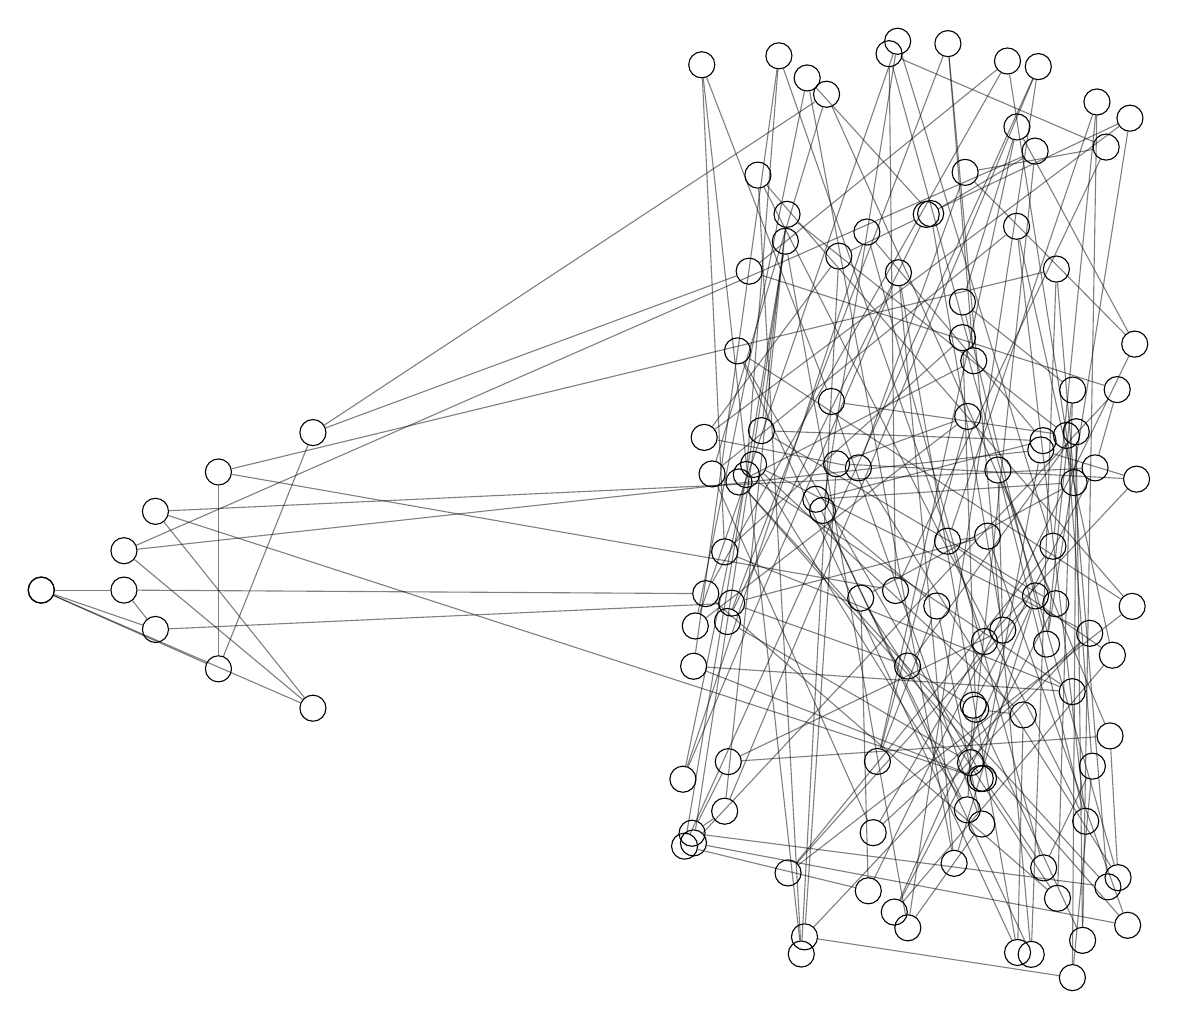
\begin{tikzpicture}[scale=1]
      \draw
        (8.715, 4.601) node[shape=circle,draw=black] (13){}
        (11.801, 2.808) node[shape=circle,draw=black] (88){}
        (9.046, 6.596) node[shape=circle,draw=black] (43){}
        (11.761, 2.209) node[shape=circle,draw=black] (110){}
        (0, 5) node[shape=circle,draw=black] (0){}
        (0, 5) node[shape=circle,draw=black] (51){}
        (12.149, 6.525) node[shape=circle,draw=black] (62){}
        (13.264, 2.064) node[shape=circle,draw=black] (99){}
        (8.99, 9.05) node[shape=circle,draw=black] (101){}
        (3.45, 7.0) node[shape=circle,draw=black] (115){}
        (8.954, 6.468) node[shape=circle,draw=black] (14){}
        (9.368, 11.785) node[shape=circle,draw=black] (22){}
        (10.378, 6.552) node[shape=circle,draw=black] (39){}
        (13.675, 1.348) node[shape=circle,draw=black] (106){}
        (12.017, 5.685) node[shape=circle,draw=black] (48){}
        (11.509, 5.621) node[shape=circle,draw=black] (118){}
        (9.471, 9.772) node[shape=circle,draw=black] (67){}
        (9.146, 7.025) node[shape=circle,draw=black] (98){}
        (11.698, 8.659) node[shape=circle,draw=black] (95){}
        (12.767, 4.314) node[shape=circle,draw=black] (114){}
        (13.383, 6.552) node[shape=circle,draw=black] (68){}
        (1.45, 6.0) node[shape=circle,draw=black] (75){}
        (11.699, 8.206) node[shape=circle,draw=black] (89){}
        (11.867, 3.487) node[shape=circle,draw=black] (107){}
        (10.407, 4.898) node[shape=circle,draw=black] (50){}
        (10.503, 1.181) node[shape=circle,draw=black] (109){}
        (8.419, 6.939) node[shape=circle,draw=black] (73){}
        (10.129, 9.241) node[shape=circle,draw=black] (74){}
        (13.144, 7.011) node[shape=circle,draw=black] (10){}
        (13.225, 0.552) node[shape=circle,draw=black] (100){}
        (11.966, 2.608) node[shape=circle,draw=black] (111){}
        (11.002, 4.035) node[shape=circle,draw=black] (25){}
        (12.892, 9.077) node[shape=circle,draw=black] (34){}
        (2.25, 6.5) node[shape=circle,draw=black] (85){}
        (12.391, 10.882) node[shape=circle,draw=black] (77){}
        (10.619, 2.824) node[shape=circle,draw=black] (83){}
        (12.906, 1.086) node[shape=circle,draw=black] (23){}
        (13.099, 7.54) node[shape=circle,draw=black] (36){}
        (11.766, 7.205) node[shape=circle,draw=black] (69){}
        (10.1, 6.604) node[shape=circle,draw=black] (97){}
        (13.02, 6.964) node[shape=circle,draw=black] (31){}
        (10.035, 7.395) node[shape=circle,draw=black] (58){}
        (1.45, 4.5) node[shape=circle,draw=black] (91){}
        (8.388, 11.671) node[shape=circle,draw=black] (18){}
        (10.767, 11.812) node[shape=circle,draw=black] (52){}
        (11.842, 7.912) node[shape=circle,draw=black] (90){}
        (13.117, 6.365) node[shape=circle,draw=black] (32){}
        (9.837, 6.154) node[shape=circle,draw=black] (87){}
        (9.45, 9.431) node[shape=circle,draw=black] (24){}
        (8.283, 1.789) node[shape=circle,draw=black] (28){}
        (10.833, 0.911) node[shape=circle,draw=black] (7){}
        (12.626, 4.926) node[shape=circle,draw=black] (76){}
        (12.848, 5.557) node[shape=circle,draw=black] (1){}
        (13.407, 11.199) node[shape=circle,draw=black] (35){}
        (11.005, 0.711) node[shape=circle,draw=black] (54){}
        (12.662, 11.648) node[shape=circle,draw=black] (72){}
        (13.546, 1.231) node[shape=circle,draw=black] (33){}
        (8.265, 1.912) node[shape=circle,draw=black] (49){}
        (9.922, 6.011) node[shape=circle,draw=black] (53){}
        (11.373, 4.798) node[shape=circle,draw=black] (82){}
        (12.211, 4.492) node[shape=circle,draw=black] (17){}
        (12.386, 9.62) node[shape=circle,draw=black] (113){}
        (8.17, 1.748) node[shape=circle,draw=black] (20){}
        (9.484, 1.408) node[shape=circle,draw=black] (9){}
        (9.101, 10.27) node[shape=circle,draw=black] (3){}
        (12.271, 11.719) node[shape=circle,draw=black] (80){}
        (12.471, 3.414) node[shape=circle,draw=black] (4){}
        (11.593, 1.53) node[shape=circle,draw=black] (27){}
        (10.886, 9.03) node[shape=circle,draw=black] (93){}
        (1.05, 5.0) node[shape=circle,draw=black] (42){}
        (8.285, 4.033) node[shape=circle,draw=black] (47){}
        (11.925, 2.606) node[shape=circle,draw=black] (105){}
        (12.572, 0.374) node[shape=circle,draw=black] (45){}
        (1.05, 5.5) node[shape=circle,draw=black] (55){}
        (3.45, 3.5) node[shape=circle,draw=black] (63){}
        (12.722, 6.898) node[shape=circle,draw=black] (30){}
        (12.694, 6.78) node[shape=circle,draw=black] (71){}
        (13.91, 6.409) node[shape=circle,draw=black] (81){}
        (10.876, 11.97) node[shape=circle,draw=black] (92){}
        (11.239, 9.771) node[shape=circle,draw=black] (94){}
        (13.826, 10.993) node[shape=circle,draw=black] (119){}
        (13.887, 8.124) node[shape=circle,draw=black] (11){}
        (11.733, 10.305) node[shape=circle,draw=black] (57){}
        (13.797, 0.743) node[shape=circle,draw=black] (15){}
        (12.73, 1.472) node[shape=circle,draw=black] (40){}
        (9.727, 11.504) node[shape=circle,draw=black] (86){}
        (11.836, 3.538) node[shape=circle,draw=black] (64){}
        (8.149, 2.598) node[shape=circle,draw=black] (2){}
        (8.306, 4.544) node[shape=circle,draw=black] (29){}
        (9.973, 11.297) node[shape=circle,draw=black] (26){}
        (12.884, 4.827) node[shape=circle,draw=black] (41){}
        (12.622, 10.575) node[shape=circle,draw=black] (12){}
        (8.842, 8.038) node[shape=circle,draw=black] (6){}
        (13.854, 4.793) node[shape=circle,draw=black] (102){}
        (13.349, 2.764) node[shape=circle,draw=black] (46){}
        (13.095, 0.078) node[shape=circle,draw=black] (65){}
        (11.944, 2.029) node[shape=circle,draw=black] (60){}
        (10.849, 4.995) node[shape=circle,draw=black] (96){}
        (8.768, 4.834) node[shape=circle,draw=black] (79){}
        (13.664, 7.546) node[shape=circle,draw=black] (44){}
        (13.093, 3.71) node[shape=circle,draw=black] (78){}
        (11.514, 11.94) node[shape=circle,draw=black] (38){}
        (11.979, 4.347) node[shape=circle,draw=black] (66){}
        (10.565, 1.919) node[shape=circle,draw=black] (70){}
        (9.652, 0.378) node[shape=circle,draw=black] (103){}
        (8.861, 6.373) node[shape=circle,draw=black] (116){}
        (13.573, 3.148) node[shape=circle,draw=black] (112){}
        (9.693, 0.596) node[shape=circle,draw=black] (59){}
        (13.315, 4.451) node[shape=circle,draw=black] (104){}
        (12.399, 0.398) node[shape=circle,draw=black] (117){}
        (8.725, 2.821) node[shape=circle,draw=black] (84){}
        (10.485, 9.547) node[shape=circle,draw=black] (108){}
        (11.295, 9.782) node[shape=circle,draw=black] (37){}
        (8.679, 2.192) node[shape=circle,draw=black] (21){}
        (8.439, 4.955) node[shape=circle,draw=black] (19){}
        (8.519, 6.475) node[shape=circle,draw=black] (5){}
        (8.679, 5.486) node[shape=circle,draw=black] (61){}
        (13.603, 4.173) node[shape=circle,draw=black] (56){}
        (13.524, 10.626) node[shape=circle,draw=black] (16){}
        (2.25, 4.0) node[shape=circle,draw=black] (8){};
      \begin{scope}[-,draw opacity=0.5]
        \draw (13) to (88);
        \draw (13) to (94);
        \draw (13) to (38);
        \draw (88) to (111);
        \draw (88) to (12);
        \draw (43) to (110);
        \draw (43) to (4);
        \draw (43) to (104);
        \draw (110) to (87);
        \draw (110) to (64);
        \draw (0) to (51);
        \draw (0) to (63);
        \draw (0) to (8);
        \draw (51) to (91);
        \draw (51) to (42);
        \draw (62) to (99);
        \draw (62) to (17);
        \draw (62) to (112);
        \draw (99) to (113);
        \draw (99) to (3);
        \draw (101) to (115);
        \draw (101) to (80);
        \draw (101) to (44);
        \draw (115) to (26);
        \draw (115) to (8);
        \draw (14) to (22);
        \draw (14) to (78);
        \draw (14) to (2);
        \draw (22) to (66);
        \draw (22) to (47);
        \draw (39) to (106);
        \draw (39) to (73);
        \draw (39) to (57);
        \draw (106) to (89);
        \draw (106) to (112);
        \draw (48) to (118);
        \draw (48) to (15);
        \draw (48) to (79);
        \draw (118) to (56);
        \draw (118) to (35);
        \draw (67) to (98);
        \draw (67) to (31);
        \draw (67) to (21);
        \draw (98) to (30);
        \draw (98) to (41);
        \draw (95) to (114);
        \draw (95) to (36);
        \draw (95) to (77);
        \draw (114) to (36);
        \draw (114) to (119);
        \draw (68) to (75);
        \draw (68) to (64);
        \draw (68) to (44);
        \draw (75) to (105);
        \draw (75) to (63);
        \draw (89) to (107);
        \draw (89) to (61);
        \draw (107) to (25);
        \draw (107) to (4);
        \draw (50) to (109);
        \draw (50) to (32);
        \draw (50) to (23);
        \draw (109) to (11);
        \draw (109) to (20);
        \draw (73) to (74);
        \draw (73) to (119);
        \draw (74) to (94);
        \draw (74) to (103);
        \draw (10) to (100);
        \draw (10) to (65);
        \draw (10) to (25);
        \draw (100) to (64);
        \draw (100) to (35);
        \draw (111) to (40);
        \draw (111) to (6);
        \draw (25) to (79);
        \draw (34) to (85);
        \draw (34) to (45);
        \draw (34) to (33);
        \draw (85) to (8);
        \draw (85) to (96);
        \draw (77) to (83);
        \draw (77) to (11);
        \draw (83) to (69);
        \draw (83) to (82);
        \draw (23) to (36);
        \draw (23) to (19);
        \draw (69) to (97);
        \draw (69) to (29);
        \draw (97) to (59);
        \draw (97) to (81);
        \draw (31) to (58);
        \draw (31) to (46);
        \draw (58) to (18);
        \draw (58) to (60);
        \draw (91) to (42);
        \draw (91) to (79);
        \draw (18) to (103);
        \draw (18) to (61);
        \draw (52) to (90);
        \draw (52) to (96);
        \draw (52) to (16);
        \draw (90) to (116);
        \draw (90) to (38);
        \draw (32) to (87);
        \draw (32) to (80);
        \draw (87) to (30);
        \draw (24) to (28);
        \draw (24) to (20);
        \draw (24) to (54);
        \draw (28) to (44);
        \draw (28) to (15);
        \draw (7) to (76);
        \draw (7) to (41);
        \draw (7) to (56);
        \draw (76) to (9);
        \draw (76) to (27);
        \draw (1) to (35);
        \draw (1) to (92);
        \draw (1) to (9);
        \draw (54) to (72);
        \draw (54) to (60);
        \draw (72) to (20);
        \draw (72) to (21);
        \draw (33) to (49);
        \draw (33) to (116);
        \draw (49) to (84);
        \draw (49) to (21);
        \draw (53) to (82);
        \draw (53) to (45);
        \draw (53) to (92);
        \draw (82) to (60);
        \draw (17) to (84);
        \draw (17) to (37);
        \draw (113) to (56);
        \draw (113) to (5);
        \draw (9) to (102);
        \draw (3) to (103);
        \draw (3) to (102);
        \draw (80) to (19);
        \draw (4) to (117);
        \draw (27) to (93);
        \draw (27) to (86);
        \draw (93) to (2);
        \draw (93) to (117);
        \draw (42) to (19);
        \draw (47) to (105);
        \draw (47) to (78);
        \draw (105) to (71);
        \draw (45) to (38);
        \draw (55) to (63);
        \draw (55) to (12);
        \draw (55) to (71);
        \draw (30) to (108);
        \draw (71) to (81);
        \draw (81) to (66);
        \draw (92) to (29);
        \draw (94) to (119);
        \draw (11) to (57);
        \draw (57) to (16);
        \draw (15) to (116);
        \draw (40) to (108);
        \draw (40) to (46);
        \draw (86) to (29);
        \draw (86) to (37);
        \draw (2) to (108);
        \draw (26) to (41);
        \draw (26) to (5);
        \draw (12) to (37);
        \draw (6) to (102);
        \draw (6) to (117);
        \draw (46) to (65);
        \draw (65) to (59);
        \draw (96) to (16);
        \draw (78) to (61);
        \draw (66) to (70);
        \draw (70) to (104);
        \draw (70) to (5);
        \draw (112) to (84);
        \draw (59) to (104);
      \end{scope}
    \end{tikzpicture}
\end{figure}

  \paragraph{Claim.} For any $v \in V^\prime$ and corresponded suggestion $c_{v}$ it holds that: $w_{E^\prime}\left( c_{v} \right) \ge \frac{1}{2}\delta_{0}\Delta$. 
  \paragraph{Proof:}By using the previews insight we get: \begin{equation*}
    \begin{split}
      w_{E^\prime}\left( c_{v} \right) &= w\left( c_{v} \right) - w_{E / E^\prime}\left( c_{v} \right) =  w\left( c_{v} \right) - w_{E / E^\prime}\left( x|_{v} \right) \\ 
      & \ge  w\left( c_{v} \right) - w\left( x|_{v} \right) \ge \frac{1}{2}w\left( c_{v} \right) = \frac{1}{2}\delta_{0}\Delta 
    \end{split}
  \end{equation*}
  $\square$

  Consider an arbitrary vertex $r \in V^\prime$, and consider the DAG obtained by the BFS walk over the subgraph $\left(V^\prime, E^\prime \right)$ starting at $r$. Denote this directed tree by $T$.

%Let $g$ be the girth of the graph and consider a layer $U$ in $T$ at height $h\left( U \right)$ satisfies the inequality $ h\left( U \right) < \frac{1}{2}g + l$ for some integer $l$.
  %\begin{adjustbox}{width=150pt}%\columnwidth}
%\begin{figure*}[t]%{width=150pt} %0.3\textwidth}

%\end{figure*}
%\end{adjustbox} 
  \paragraph{Claim.} The size of $T$ is at least:
  \begin{equation*}
    \begin{split}
      |T| & \ge \left( \frac{1}{4}\delta_{0} - \frac{\lambda}{\Delta} \right)n 
    \end{split}
  \end{equation*}
  \paragraph{Proof:} By the fact that for any $v \in T$ the degree of $v$ is at least $\frac{1}{2}\delta_{0}\Delta$ we have that: $E\left( T,T \right) \ge \frac{1}{2}\cdot \frac{1}{2}\delta_{0}\Delta |T|$. Combine the Mixining Expander Lemma we obtain:
  \begin{equation*}
    \begin{split}
      \frac{1}{4}\delta_{0}\Delta |T| & \le \frac{\Delta}{n}|T|^2  + \lambda|T| \\ 
      \Rightarrow & \left( \frac{\Delta}{n}|T| + \lambda -  \frac{1}{4}\delta_{0}\Delta \right)|T| \ge 0 \\ 
      \Rightarrow & |T| \ge \left( \frac{1}{4}\delta_{0} - \frac{\lambda}{\Delta} \right)n 
    \end{split}
  \end{equation*}
  $\square$
 %
 %  \paragraph{Claim.} There is a constant $\gamma > 0 $ such for any  $S \subset T$ it holds that:  
 %  \begin{equation*}
 %    \begin{split}
 %      \frac{\lambda}{\Delta} \le \gamma\left( 1 - \frac{1}{2}\delta_{0} \right)\frac{|S|}{|T|}
 %    \end{split}
 %  \end{equation*}
 %
 %  \paragraph{Proof.} Recall that the second largest eigenvalue 
 %
 %  Denote by $x|_{U}$ the bits of $x\in C$ correspond to the edges connected to at least one vertex in $U$. And denote by $w_{E/E^{\prime}}\left( x|_{U} \right)$ the weight induced by the $x|_{U}$ over the edges in $E/E^\prime$.

  \paragraph{Claim.} Suppose that $G$ is an expander graph with a second eigenvalue $\lambda$, then For any layer $U$ there exist a layer $U^{\prime}$ such that:
  \begin{equation*}
    \begin{split}
      (1) & \ \ |U^{\prime}| \ge |U| \\
      (2) & \ \ w_{E/E^{\prime}}\left( x|_{U^{\prime}} \right)  \ge\Delta|U^{\prime}|\left( \delta_{0}-\frac{2}{3}-\frac{2\lambda}{\Delta} \right)
    \end{split}
  \end{equation*}
  \paragraph{Proof:} Consider layer $U$ and denote by $U_{-1}$ and $U_{+1}$ the preceding and the following layers to $U$ in $T$. It follows from the expander mixing lemma that:
  \begin{equation*}
    \begin{split}
      w_{E/E^{\prime}}\left( x|_{U} \right) & \ge \delta_{0}\Delta|U| -w\left( E(U_{-1} \bigcup U_{+1} ,U)  \right) \ge \\ 
      & \delta_{0}\Delta|U| -\left( E(U_{-1} \bigcup U_{+1} ,U)  \right) \\ 
      &  \delta_{0}\Delta|U| - \Delta\frac{|U||U_{-1}|}{n} - \Delta\frac{|U||U_{+1}|}{n} \\
      & -\lambda\sqrt{|U||U_{-1}|} - \lambda\sqrt{|U||U_{+1}|}
    \end{split}
  \end{equation*}

  \paragraph{Claim.} We can assume that $|U| \ge |U_{-1}|, |U_{+1}|$. 
  \paragraph{Proof:} Suppose that $|U_{+1}| > |U|$, so we could choose $U$ to be $U_{+1}$. Continuing stepping deeper till we have that $|U| > |U_{+1}|, |U_{-1}|$. Simiraly, if $|U| > |U_{+1}|$ but $|U_{-1}| > |U|$, the we could take steps upward by replacing $U_{-1}$ with $U$. At the end of the process, we will be left with $U$ at a size greater than the initial layer and $|U| > |U_{+1}|, |U_{-1}|$ $\square$

  Using the the claim, we have that $\left( |U_{+1}| + |U_{-1}| \right)/n <\frac{2}{3} $ and therefore:
  \begin{equation*}
    \begin{split}
      w_{E/E^{\prime}}\left( x|_{U} \right) & \ge \left( \delta_{0} - \frac{2}{3} - \frac{2\lambda}{\Delta} \right) \Delta |U| \ \  \square 
    \end{split}
  \end{equation*}

  That immediately yields the following: let $U_{\text{max}} = \text{arg} \max_{U \text{ layer in }  T } |U|  $  then: 
  \begin{equation*}
    \begin{split}
      |x| \ge  w_{E/E^{\prime}}\left( x|_{U_{\text{max}}} \right) \ge \left( \delta_{0} - \frac{2}{3} - \frac{2\lambda}{\Delta} \right)\Delta |U_{\text{max}}|
    \end{split}
  \end{equation*}
  \paragraph{Claim.} Consider again the maximal layer $U_{\max}$ then: 
  \begin{equation*}
    \begin{split}
      w_{E/E^{\prime}}\left( x \right) \ge \left( \delta_{0} - \frac{|U_{\max}|}{n} - \frac{\lambda}{\Delta} \right) \Delta|T| 
    \end{split}
  \end{equation*}
  \paragraph{Proof.} Similarly to above, now we will bound the weight that all the nodes in $T$ induce over $E/E^{\prime}$. Denote by $U_{0}, U_{1} .. U_{m}$ the layers of $T$ ordered corresponded to their height, thus we obtain: 
  \begin{equation*}
    \begin{split}
      w_{E/E^{\prime}}\left( x \right) & \ge \delta_{0}\Delta|T| - \sum_{i\in [m]}{ w \left( E\left( U_{i}, U_{i+1}  \right) \right)  } \\ 
      \ge & \delta_{0}\Delta|T|  - \sum_{i \in [m]}{ E\left( U_{i}, U_{i+1}  \right)  } \\ 
      \ge & \delta_{0}\Delta|T|  -  \sum_{i \in [m]}{ \frac{\Delta}{n}|U_{i}| |U_{i+1}| + \lambda \sqrt{ |U_{i}| |U_{i+1}|} }\\ 
      \ge & \delta_{0}\Delta|T|  -  \sum_{i \in [m]}{ \frac{\Delta}{n}|U_{i}| |U_{i+1}| + \lambda \frac{ |U_{i}|+ |U_{i+1}|}{2 } }\\ 
      \ge & \delta_{0}\Delta|T|  - \frac{\Delta}{n}|T||U_{\max}| -  \lambda |T| \\ 
      \ge & \left( \delta_{0} - \frac{|U_{\max}| }{n}-  \frac{\lambda}{\Delta} \right) \Delta|T| 
    \end{split}
  \end{equation*}
  $\square$
  \paragraph{Proof of Theorem 1.} Consider the size of the maxiaml layer $|U_{\max}$ and sepearte to the following two cases. First, consider the case that $|U_{\max}| \ge  \alpha n $ in that case it follows immedily that if $\delta_{0} > \frac{2}{3} - \frac{2\lambda}{\Delta}$ there exists $\alpha^{\prime} > 0 $ such that:  
  \begin{equation*}
    \begin{split}
      |x| \ge \left( \delta_{0} - \frac{2}{3} - \frac{2}{\lambda}\Delta \right)\Delta|U_{\max}| \ge  \alpha^{\prime} n 
    \end{split}
  \end{equation*}
  So, it is lefts to consider the second case in which $ |U_{\max}| < \alpha n $ in that case, we have from the second inequality that: 

  \begin{equation*}
    \begin{split}
      |x| & \ge  w_{E/E^{\prime}}\left( x \right)  \ge \left( \delta_{0} - \frac{|U_{\max}|}{n} - \frac{\lambda}{\Delta} \right) \Delta|T| \\ 
      & \ge \left( \delta_{0} - \alpha - \frac{\lambda}{\Delta} \right) \Delta|T| 
    \end{split}
  \end{equation*}
  Setting $\alpha \ge \frac{2}{3}$ we complete the proof $\square$

  Unfortunately, Singelton bound doesn't allow both $\delta_0 > \frac{2}{3}$ and $\rho_0 \ge \frac{1}{2}$, so in total, we prove the existence of code LDPC code which is good in terms of testability and distance yet has a zero rate. In the following subsection, we will prove (\ctt{sec 3.4, which currently is a failure}) that one can overcome this problem by requiring only half of the vertices to restrict their local view to be codewords of high relative distance. 
%\subsection{ Good LTC Which Is Almost LDPC. } 
%To overcome the vanishing rate issue, we are going to consider the graphs family in which the maximal layer of BFS scanning couldn't exceed a linear  

 %
 %  \begin{equation*}
 %    \begin{split}
 %      \left( 1 - \frac{1}{2}\delta_{0} \right)\Delta |T| \ge \left( \delta_{0} - \frac{|U_{\max}|}{n} - \frac{\lambda}{\Delta} \right) \Delta|T| 
 %    \end{split}
 %  \end{equation*}

  \subsection { Overcoming The Vanishing Rate. } 
  Consider the following code; instead of associating each edge with pair of checks, let's define the vertices to be the checks of small codes over $q \in [0,1]$ fraction of their edges. That is, now each vertex defines only $\left( 1 - \rho_{0} \right)q\Delta$ restrictions. Hence, the rate of the code is at least:   
  \begin{equation*}
    \begin{split}
      \rho\frac{1}{2}\Delta n & \ge \frac{1}{2}\Delta n - \left(1 - \rho_{0} \right)q\Delta n \\
      \Rightarrow \rho & \ge \left(  2\rho_{0} + \left( \frac{1}{q}  - 2  \right)  \right)q \\ 
      \rho_{0} & \ge  1 - \frac{1}{2q} 
    \end{split}
  \end{equation*} for example, if $q = 2/3$, then for having constant rate, it is enough to ensure that $ \rho_{0} \ge 1 - \frac{3}{4} = \frac{1}{4}$.

 \paragraph{Intuition For Testability.} Before expand the construction let's us justifiy why one should even expects that removing constrainsts preserves testability. Assume that is gurnted that the lower bound of the flux on the trivial vertices remains up to multiplication by the fraction factor $q$, or put it diffrently, one could just stick $q$ in every inequalitiy without lose correcntess, Then: 
  \begin{equation*}
    \begin{split}
      w_{E/E^{\prime}}\left( x|_{U} \right) & \ge  \delta_{0}q\Delta|U| -qw\left( E(U_{-1} \bigcup U_{+1} ,U)  \right) \\ 
      \Rightarrow |x| & \ge \left(  \delta_{0} - \frac{2}{3} - \frac{2\lambda}{\Delta} \right) q \Delta|U_{\max}|
    \end{split}
  \end{equation*}
  As you can see, ireducable words of the disagreement have a linear weight, dispite that the orignal code has non-vanish rate.     
  
  \paragraph{Theorem 1+.} There exist a constant $\alpha > 0 $ and infinite familiy of codes which satesfies Theroem 1 and also good.
  \paragraph{}

  Yet, We still require more to prove a linear distance. 
  By repeating on the ~\cref{theorem*:Sing} \emph{Singleton Bound} proof it follows that the small code $\tilde{C_{0}}$ obtained by ignoring arbitrary $ \left( q - \frac{1}{2} \right) \Delta $ coordinates yield a code with distance: 
  \begin{equation*}
    \begin{split}
      \left( \delta_{0} - \left( q - \frac{1}{2} \right) \right)\Delta
    \end{split}
  \end{equation*}
  So assume that we could engineer an expander family such that the graphs obtained by removing $\frac{1}{2}$ of the edges connected for each vertex result also expanders, and in addition, regarding $\tilde{C_{0}}$ each edge is checked by both vertices on its support. Namely, a good Tanners Code could be defined on the restricted graphs; Then, any string that satisfies the original checks also has a linear weight. To achieve this property, we will restrict ourselves to a particular family of Cayley Graphs.  
  \paragraph{Definion. Testability-Tanner-Code.} Let $q > \frac{1}{2}$ and let $J$ be a geneator set for group $\Gamma$ such that $|J| = \Delta$, $q | \Delta $, $J$ closed for inverse, and there exist subset of $J$, denote it by, $J^{\prime}$ such that $J^{\prime}$ is a generator set of $\Gamma$ and $|J^{\prime}| = \frac{1}{2}\Delta$. Let $C_{0}$ be a code with parameters $C_{0} = q\Delta \left[1, \rho_{0}, \delta_{0}\right]$. For any vertex assoicate a subset $\Jvv \subset J/J^{\prime}$ at size: 

  \begin{equation*}
    \begin{split}
      |\Jvv| = \left( q - \frac{1}{2} \right)\Delta \Rightarrow |\Jvv \cup J^{\prime}| = q\Delta
    \end{split}
  \end{equation*}
  Define the code $\mathcal{T}\left(J, q , C_{0}\right)$ to be the subspace such that any vertex's local view over the edges defined by $\Jvv \cup J^{\prime}$ is a codeword of $C_{0}$. In addition, let's associate a code $\Cvv$ obtained for any vertex by ignoring the bits supported on the $\Jvv$ coordinates. Notice that code defined by requiring that the local view of any vertex $v$ of \emph{Cayley}$\left(\Gamma, J^{\prime} \right)$ is a codeword of $\Cvv$ is a TannerCode. Denote it by $ \tilde{\mathcal{T}}\left(J, q ,C_{0}\right)$.   

  \paragraph{Lemma.} Let $J$ be defined as above such that both \emph{Cayley}$\left( \Gamma, J \right)$, \emph{Cayley}$\left( \Gamma, J^{\prime} \right)$ are expanders with algebric expansion greater then $\lambda$ and $C_0$ with the parameters $\rho_{0} > 1 - \frac{1}{2q}$ and $ \delta_{0} - \left( q - \frac{1}{2} \right) > \lambda$. Then the code $\mathcal{T}\left(J, q ,C_{0}\right)$ is a good code. 
  \paragraph{Proof.} We have already proven that the code has a positive rate. Consider a codeword $x$ and denote by $x^{\prime}$ the restriction of $x$ to \emph{Cayley }$\left( \Gamma, J^{\prime}  \right)$ which is a codeword of $\tilde{C} = \tilde{\mathcal{T}}\left(J, q ,C_{0}\right)$. But $\tilde{C}$ is a Tanner Code such that any vertex sees at least $ \tilde{\delta_{0}} \Delta := \left(\delta_{0} - \left( q - \frac{1}{2}   \right) \right)\Delta $ nontrivial bits, Therefore as the expansion of the graph \emph{Cayley}$\left( \Gamma, J^{\prime} \right)$ is lower than $\tilde{\delta}\Delta$ than any subset $S$ of $V$ at the size at most $|S|/|V| < \tilde{\delta_{0}} - \lambda / \Delta $  must contain at least one vertex that sees less than  $\tilde{\delta}\Delta$ nontrivial bits, In contradiction for the fact that $x^{\prime} \in \tilde{C}$. $\square$ 

  \paragraph{Claim. Existence of such \emph{Cayley's}.} Let $S$ be a generator set such that \emph{Cayley}$\left( \Gamma , S \right)$ has a second largest eigenvalue greater then $\lambda$, And consider an arbitray group element $g \in \Gamma$ such that $gSg^{-1}$ disjointness to $S$ \ctt{ remove the disjointness requirment}. Denote by $S_{g}$ the set $gSg^{-1}$. Then the second eigenvalue of the graph obtained by $\left( \Gamma, S \right) \cup \left( \Gamma, S \right)$ is at most $2\lambda$. 
  \paragraph{Proof.} Denote by $G,G^{\prime}$ the \emph{Cayley} graphs coressponding to $S$, $S_{g}$, for conviniet we will use the notation of $\sum_{v\sim_{G} u}$ to denote a summation over all the neighboors of $v$ in the graph $G$. Let $A_{G^{\prime}}$ be the adjacency matrix of $G^{\prime}$. Recall that $G^{\prime}$ is a  $\Delta$ regular graph, and therefore the uniform distribution $\mathbf{1}$ is the eigenstate with the maximal eigenvalue, and the second eigenvalue is given by the min-max principle: 
  \begin{equation*}
    \begin{split}
      & \max_{f \perp \mathbf{1}} { \frac{f^{\top}A_{G^{\prime}} f  }{ f^{\top}f}} = \max_{f \perp \mathbf{1}} { \sum_{v}  \sum_{u\sim_{G^{\prime}} v}\frac{f\left( u \right) f \left( v \right)  }{ f^{\top}f}} \\
      =  & \max_{f \perp \mathbf{1}} { \sum_{v}\sum_{\tau \in S} \frac{f\left( g\tau g^{-1} v \right) f \left( v \right)  }{ f^{\top}f}} \\ = & \max_{f \perp \mathbf{1}} { \sum_{gv} \sum_{\tau \in S}\frac{f\left( g\tau g^{-1} gv \right) f \left( gv \right)  }{ f^{\top}f}} \\  
      = & \max_{f \perp \mathbf{1}} { \sum_{gv}\sum_{\tau \in S}\frac{f\left( g \tau v \right) f \left( g v \right)  }{ f^{\top}f}} \\  = & \max_{f \perp \mathbf{1}} { \sum_{gv}\sum_{ u\sim_{G} v }\frac{f\left( gu \right) f \left( gv \right)  }{ f^{\top}f}} \\
         \end{split}
  \end{equation*}
  As for any function $f : V \rightarrow \mathbb{R} $ one could define a function $f^{\prime} : E \rightarrow \mathbb{R} $ such that $f^{\prime}\left( v \right) = f\left( v \right) $ and $f^{\prime}$ preservs the norm:    
  \begin{equation*}
    \begin{split}
     &  f^{\prime \top}f^{\prime}   = \sum_{v \in V}f^{\prime}\left( v \right)f^{\prime}\left( v \right)   =   \sum_{v \in V } f^{\top}\left( vg \right)f\left( vg \right) = f^{\top}f \\
     \Rightarrow  &  \max_{f \perp \mathbf{1}} { \frac{f^{\top}A_{G^{\prime}} f  }{ f^{\top}f}} =\max_{f \perp \mathbf{1}} { \sum_{gv}\sum_{ u\sim_{G} v }\frac{f\left( gu \right) f \left( vg \right)  }{ f^{\top}f}} 
    \end{split}
  \end{equation*}
  By the Interlacing Theorem, \cite{HAEMERS1995593} the second eigenvalue of any subgraph of $G^{\prime}$ is less than the $\lambda^{\prime}$, In particular, the eigenvalue of the graph obtained by taking the edges that are associated with elements of the $ S_{g} / S $, denote that subgraph by $G^{\prime}_{ / S}$. Because $S_{g} / S \cap S = \emptyset $, we have that the edges sets of $G, G^{\prime}$ are disjointness sets. Hence the adjacency matrix of the graphs union equals the sum of their adjacency matrices. So in total, we obtain that:  
    \begin{equation*}
    \begin{split}
      \lambda^{\prime} &= \max_{f \perp \mathbf{1}} { \frac{f^{\top} \left( A_{G} + A_{G^{\prime}_{/S}} \right) f  }{ f^{\top}f}} \\
      & \le  \max_{f \perp \mathbf{1}} { \frac{f^{\top}A_{G} f  }{ f^{\top}f}} +  \max_{f \perp \mathbf{1}} { \frac{f^{\top}A_{G^{\prime}_{/S}} f  }{ f^{\top}f}} \\
      & \le \lambda + \lambda = 2\lambda
    \end{split}
  \end{equation*} 
  $\square$ 
  \paragraph{Claim.} If $\Delta$ is a constant greater than two, and $G$ is a $\lambda$-algebric expander with girth at length $\Omega\left( \log n \right)$, then it there exists a $g \in \Gamma$ such that $S_{g}\cap S = \emptyset$.  
  \paragraph{Proof.} As $\Delta > 2 $ there must be at least two different elements $s_{1},s_{2} \in S$  such that $s_{1} \neq s_{2}, s_{2}^{-1}$. Pick $g = s_{1}s_{2}$. Now assume through contradiction that there also exists $s,t \in S$ such that $gsg^{-1} = r \Rightarrow gs = rg$ and notice that the fact that $s_{1}\neq s_{2}^{-1}$ guarantees that both terms are a product of $3$ element group. Therefore either that there is a $6$-length cycle in the graph, Or that there is element-wise equivalence, namely $s_{1} = r, s_{2} = s_{1}, s=s_{2}$. The first case contradict the lower bound on the expander girth, which is at least $\Omega \left( \log_{\Delta}(n) \right)$, while the other stand in contradiction to the fact that $s_{1} \neq s_{2}$ $\square$  
  \paragraph{Remark. Regarding Quantum Codes.} Notice that any complex designed to hold CSS qLDPC codes must have constant length cycles. Otherwise, the distance of $C_{x}$ will not be constant, and therefore the condition $H_{x}H_{z}^{\top} =0$ could be satisfied only if $H_{z}$ is not a constant row-weight matrix, Put differently $C_{z}$ is not an LDPC code. Consequently, any trial to generalize the construction for obtaining quantum codes must not rely on that claim.    

  \paragraph{Remark. Note On Random Construction.} One might wondring if using \emph{Cayley} is necssery. We conjecure that there is a constant $c > 0$ such that sampling pair of  $\left( 1 + c \right)\frac{1}{2}\Delta$ regulr random graphs, and than take the anti-symatry union of them might also obtain a good expander such that each of the reseuide part also has good expansion with heigh probability.  
  \paragraph{Lemma.} \ctt{Rewrite}. Consider the graph $G$ as defind above (direct subset of \emph{Cayley} graph) and let $S$, $T$ be subsets of the vertices. Then the flux of $S$ over $T$ is at most: 
  \begin{equation*}
    \begin{split}
      E_{G^{\prime}}(S,T) \le \frac{1}{2} \Delta\frac{|S||T|}{n} + \lambda\sqrt{|S||T|} 
    \end{split}
  \end{equation*} 

  \paragraph{Proof.} The only edges that can interferce are the edge defined by $J^{\prime}$. Therefore it's enough to use the mixing expander lemme on the $\frac{1}{2}\Delta$-regular graph. $\square$


  \paragraph{Proof of Theorem 1+.} Noitce that $\frac{1}{2} < \frac{2}{3} = q$, Thus reapting exactly over proof above obtains that: 
  \begin{equation*}
    \begin{split}
      w_{E/E^{\prime}}\left( x|_{U_{\text{max}}} \right) \ge \left( \delta_{0} - \frac{2}{3} - \frac{1}{q}\frac{2\lambda}{\Delta} \right)q\Delta |U_{\text{max}}|
    \end{split}
  \end{equation*}
  Choseing $J$ such that \emph{Cayley}$\left( \Gamma, J \right)$ is ramnujan provid that $ \frac{2\lambda}{\Delta q}$ sacle as $\Theta\left( \frac{1}{\sqrt{\Delta}} \right)$. That close the case in which there is a linear size layer of nontrival suggestions. In other case, in which any such layer is at size less than $\alpha^{\prime}n$ ( $\alpha^{\prime} = \left( \delta_{0} - \left( q - \frac{1}{2} \right) \right)$ ? ) then we obtain the testbility for free $\square$
      \section{Good Quantum Codes, logaritmic-check-weight.} 
In the following section we will construct a family of complexes on which we will define a pairs of Tanner Codes, evently, they will used to compose a CSS pairs of good quantum codes.  
  \paragraph{Inifinte Family Of Tanner Quantum Codes.} 
  Let $p$ be a prime and $\delta \in \left( 0,1 \right)$. Consider the Cayly graphs obtained by taking uniformly a $c\left( \delta \right)\log n$ generators of the cyclic group at order $p$, denote that set by $S$. It was shown by N.Alon \ctt{cite Noga} that with high probability that process yield a Graph with $\delta$-algebric expansion. Now, consider the double cover of that graph and denote it by $G = \left( V = V^{+} \cup V^{-},E \right)$. And define the folowing graph denoted by $\Gamma^{\pm} = \left(V^{\pm}, E^{\prime}\right)$:
  \begin{equation*}
    \begin{split}
      \left( \left(u , \pm  \right), \left( v, \pm \right) \right) \in  E^{\prime} \Leftrightarrow \exists a\neq b \in S \ s.t \ abu = v     
    \end{split}
  \end{equation*}
     

  \section{Decoding and Testing}
  For completeness, we show exactly how Theorem 1 implies testability. The following section repeats Leiverar's and Zemor's proof \cite{leverrier2022quantum}. Consider a binary string $x$ that is not a codeword. The main idea is the observation that the number of bits filliped by (any) decoder, while decoding $x$, bounds the distance $d\left( x, C \right)$ from above. In addition, the number of positive checks in the first iteration is exactly the number of violated restrictions.
%\begin{figure*}[h]
%\begin{adjustbox}{width=\textwidth}
  \begin{definition}Let $L = \{L_{i}\}^{2|E|}_{0}$  be a series of $2|E|$. Such that for each vertex $ v \in V$ $\sum_{ e = \{u,v\} }{ L_{e_v} } \in C_{0}$. We will call $L$ a \textit{Potential list} and refer to the $e_{v}$'the element of $L$ as a suggestion made by the vertex $v \in V$ for the edge $e \in E$. Sometimes we will use the notation $L_{v}$ to denote all the $L$'s coordinates of the form $ L_{e_{v}} \forall e \in \text{Support} \left( v \right) $. Define the \textit{Force} of $L$ to be the following sum $  F\left( L \right) = \sum_{e = \{v,u\} \in E }{ \left(L_{e_v} + L_{e_u}\right) }$ and notice that $ F\left( L \right) \in C_{\oplus}$. And define the \textit{state} $S(L) \subset \mathbb{F}^{|E|}_{2}$ of $L$ as the vector obtained by choosing an arbitrary value from $ \{ L_{e_v}, L_{e_u} \}$ for each edge $e \in E$.  
  \end{definition}
  \begin{claim} \label{claim:pot} Let $L$ be the Potential list. If $F(L)=0$ then $S(L)\in C$. \end{claim}
  \begin{proof} Denote by $\phi\left( e \right) \subset \{ L_{e_v}, L_{e_u} \}$ the value which was chosen to $e = \{v,u\} \in E$. By $F\left(L\right) = 0$ , it follows that $ L_{e_v} + L_{e_u} = 0 \Rightarrow L_{e_v} = L_{e_u} = \phi\left( e \right) $ for any $e \in E$. Hence for every $v\in V$ we have that $ S\left( L \right)|_{v} = \sum_{u \sim v}{ \phi\left( \{v,u\} \right) } =  \sum_{u \sim v}{ L_{e_v }} \in C_{0}$ $ \Rightarrow S\left( L \right) \in C$   
  \end{proof}
  The decoding goes as follows. First, each vertex suggests the closet $C_{0}$'s codeword to his local view. Those suggestions define a Potential list, denote it by $L$, then if $F\left( L \right) <\tau$, by Theorem 1, one could find a suggestion of vertex $v$ and a codeword $c_v$ such that updating the value of $L_{v} \leftarrow L_{v} + c_{v}$ yields a Potential list with lower force. Therefore repeating the process till the force vanishes, obtain a Potential list in which its state is a codeword. 
  \begin{definition} Let $\tau > 0, f : \mathbb{N} \rightarrow \mathbb{R^{+}}$, and consider a Tanner Code $C = \mathcal{T}\left( G, C_{0} \right)$. Let us Define the following decoder and denote it by $\mathcal{D}$.  
  \end{definition}

  \begin{algorithm}[h]
    \caption{Decoding}
    \label{alg:three}
    \KwData{ $x \in \mathbb{F}_{2}^{n}$ }
    \KwResult{ $\arg\min {\left\{  y \in C : |y + x|  \right\} }$ if $d(y,C) < \tau $ and False otherwise. }
    $ L \leftarrow \text{Array} \{ \} $\\
    \For { $ v \in V$} {
      $c^{\prime}_{v} \leftarrow \arg\min {\left\{  y \in C_{0} : |y + x|_{v} |  \right\} } $\\
      $ L_{v} \leftarrow c^{\prime}_{v}$
    }
    $ z \leftarrow \sum_{v \in V}{c^{\prime}_{v}} $\\
    \eIf{ $ |z| < \tau \frac{n}{f\left( n \right)} $}{
      \While{ $|z| > 0$ }{
	find $v$ and $c \in C_{0}$ such that $|z + c_{v}| < |z|$\\
	$z \leftarrow z + c_{v}$ \\
	$ L_{v} \leftarrow  L_{v} + c_{v}$
      }
    }{
      reject. 
    }
    \Return  $S(L) $

  \end{algorithm}

  \begin{theorem}
Consider a Tanner Code $C = [n, n\rho, n\delta]$ and the corresponding disagreement code $C_{\oplus}$. Suppose that for every codeword $z \in C_{\oplus}$ such that $|z| < \frac{\tau^{\prime} n}{f\left(n\right)}$, there exists a vertex $v$ and a suggestion for $v$ which is another codeword $y \in C_{\oplus}$ such that $|z + y| < |z|$. Set $\tau \leftarrow \frac{\tau^{\prime}}{6 \Delta} \delta$ then.

  \begin{enumerate}
    \item $\mathcal{D}$ corrects any error at a weight less than $\tau n / f\left(n\right)$.   
    \item $C$ is $f\left( n \right)$ testable code.
  \end{enumerate}
\end{theorem}

\begin{proof} So it is clear from the claim \cref{claim:pot} above that if the condition at line (6) is satisfied, then $\mathcal{D}$  will converge into some codeword in $C$. Hence, to complete the first section, it left to show that $\mathcal{D}$ returns the closest codeword. Denote by $e$ the error, and by simple counting arguments; we have that $\mathcal{D}$ flips at most:  
  \begin{equation*}
    \begin{split}
      d_{\mathcal{D}}\left( x, C \right) & \le 2|e|\Delta + \tau \frac{n}{f\left( n \right)}\Delta
    \end{split}
  \end{equation*}
  bits. Hence, by the assumption, 
  \begin{equation*}
    \begin{split}
      d_{\mathcal{D}}\left( x, C \right) & \le 3\Delta \tau \frac{n}{f\left( n \right)} \le 3\Delta \tau\delta n < \frac{1}{2} \delta n  
    \end{split}
  \end{equation*}
  Therefore the code word returned by $\mathcal{D}$ must be the closet. Otherwise, it contradicts the fact that the relative distance of the code is $\delta$.
  To obtain the correctness of the second section, we will separate when the conditional at the line (5) holds and not. And prove that the testability inequality holds in both cases. 
  Let $x \in \mathbb{F}_{2}^{n}$ and consider the running of $\mathcal{D}$ over $x$. Assume the first case, in which the conditional at line (5) is satisfied. In that case, $\mathcal{D}$ decodes $x$ into its closest codeword in $C$. Therefore:
  \begin{equation*}
    \begin{split}
      d\left( x, C \right) \le & \ d_{D} \left( x, C \right) \le m\xi\left( x \right)\Delta +  |z|\Delta  \\ \le &  \  m\xi\left( x \right)\Delta + m\xi\left( x \right)  \Delta^{2} \\ 
      \frac{d\left( x, C \right)}{n} \le & \  \kappa_{1} \xi\left( x \right)    
    \end{split}
  \end{equation*}
  Now, consider the other case in which: $ |z| \ge \tau \frac{n}{f\left( n \right)}  $.
  \begin{equation*}
    \begin{split}
      \frac{d\left( x, C \right)}{n} & \le 1 \le \frac{|z|}{\tau n}f\left( n \right) \le \frac{m}{n} \frac{1}{\tau} \Delta \xi\left( x\right)f\left( n \right) \\ & \le \kappa_{2} \xi\left( x \right)f\left( n \right)  
    \end{split}
  \end{equation*}
  Picking $ \kappa \leftarrow \max \{ \kappa_{1}, \kappa_{2} \}$ proves $f\left( n \right)$-testability
\end{proof}


  %\end{adjustbox}
%\end{figure*}
%\end{multicols*}
\printbibliography 
\end{document}

 



